\section{Programming Methodologies} \label{sec:programming}

In this section we propose two programming methodologies targeted very differently. The fast MLC programming methodology is devised for ReRAM memory when performance is a very critical and seldom soft error can be tolerated. This assumption holds true for main memory in traditional memory hierarchy. DRAM-based main memory are usually designed with ECC to tackle particle-strike soft error. More importantly, most of the data in main memory does not have to be "stored" for a long time as either they will be updated frequently or they will be useless without future accesses. The reliable MLC programming methodology is more suitable for storage system where data integrity is extremely important. For example, the data in SSD or USB driver may need to be stored for years. Moreover, even microsecond-level write latency can be hidden by large block size in conventional NAND flash product, maintaining an acceptable bandwidth. We will use 3-bit MLC cell as illustrations in this section since 8-level stable states have been widely reported in experimental data for MLC ReRAM. We denote the three bits in a ReRAM cell as $D_2D_1D_0$ where $D_2$ is the most significant bit (MSB) and $D_0$ is the least significant bit (LSB). "111" denotes the lowest LRS resistance while "000" denotes the highest HRS resistance.

\subsection{Fast MLC programming methodology}

\begin{figure}[t]
\centering
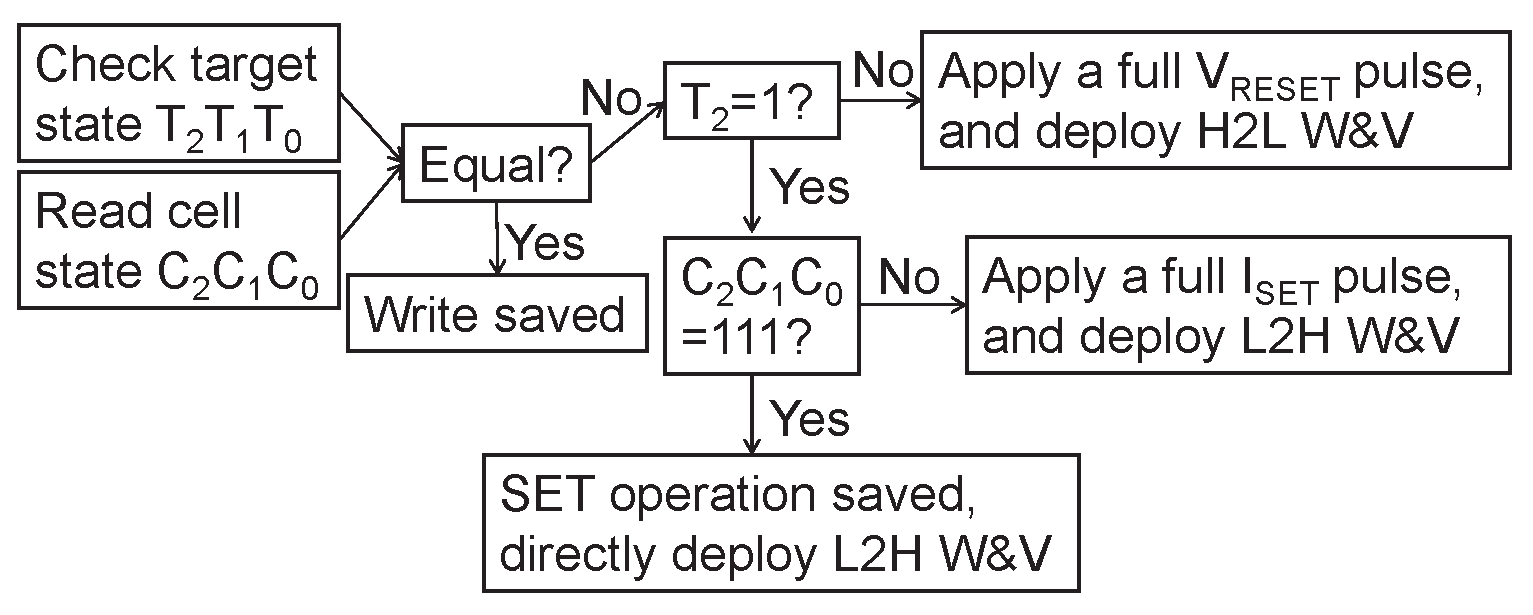
\includegraphics[width=0.48\textwidth]{fig/fastprog}
\vspace{-10pt}
\caption{Flowchart of fast programming methodology}
\label{fig:fastprog}
\vspace{-15pt}
\end{figure}

The goal of the fast MLC programming methodology is to reduce the average write latency by avoiding the states that require large number of iteration steps in either H2L or L2H programming. The flowchart of the proposed programming methodology is illustrated in Figure~\ref{fig:fastprog}. Before the actual programming starts, current state of the cell $C_2C_1C_0$ is first read out and compared with the target state $T_2T_1T_0$ to be programmed. If they are equal, the programming was skipped. Otherwise it is required to identify whether the target state easier to reach from HRS or LRS, which can be simply achieved by checking the MSB of the target state: $T_2=0$ means the target state is relative high resistance and may require smaller number of iteration steps in H2L programming. In that case, we apply a full RESET voltage across the cell and push it to the highest level of HRS and then deploy H2L programming. Note that read was first performed immediately after the full RESET operation and the first verification result indicates whether $T_2T_1T_0=000$ or not. If the $T_2=1$ then L2H programming may be preferred. Here an additional comparison is made to to save possible SET operation if original cell state is already in lowest level of LRS. If $C_2C_1C_0=111$ then we can begin L2H programming without a complete SET operation first, otherwise a full SET current pulse is applied on the cell first. So far, the first state-aware programming methodology is devised to achieve fast MLC programming speed by the speculation of both the target state and the original cell state. However, some programmed states by the fast programming methodology may be somewhat vulnerable to retention failure. For example, if $T_2T_1T_0=110$ the programmed state is achieved by slightly rupturing the strongly formed CFs and LRS retention failure is likely to occur in the cell. In contrast, if $T_2T_1T_0=001$ then weak CFs are reconstructed from HRS and HRS retention failure is likely to occur in the cell. Fortunately, the probability of retention failure under normal operation temperature of ReRAM is very small (smaller than the probability of DRAM soft error[??]). Therefore, the programming methodology can be widely adopted in MLC ReRAM application except for the scenario where the requirement of data retention is extremely restricted. Hence the second MLC programming methodology with excellent reliability is also proposed.

\subsection{Reliable MLC programming methodology}
\begin{figure}[t]
\centering
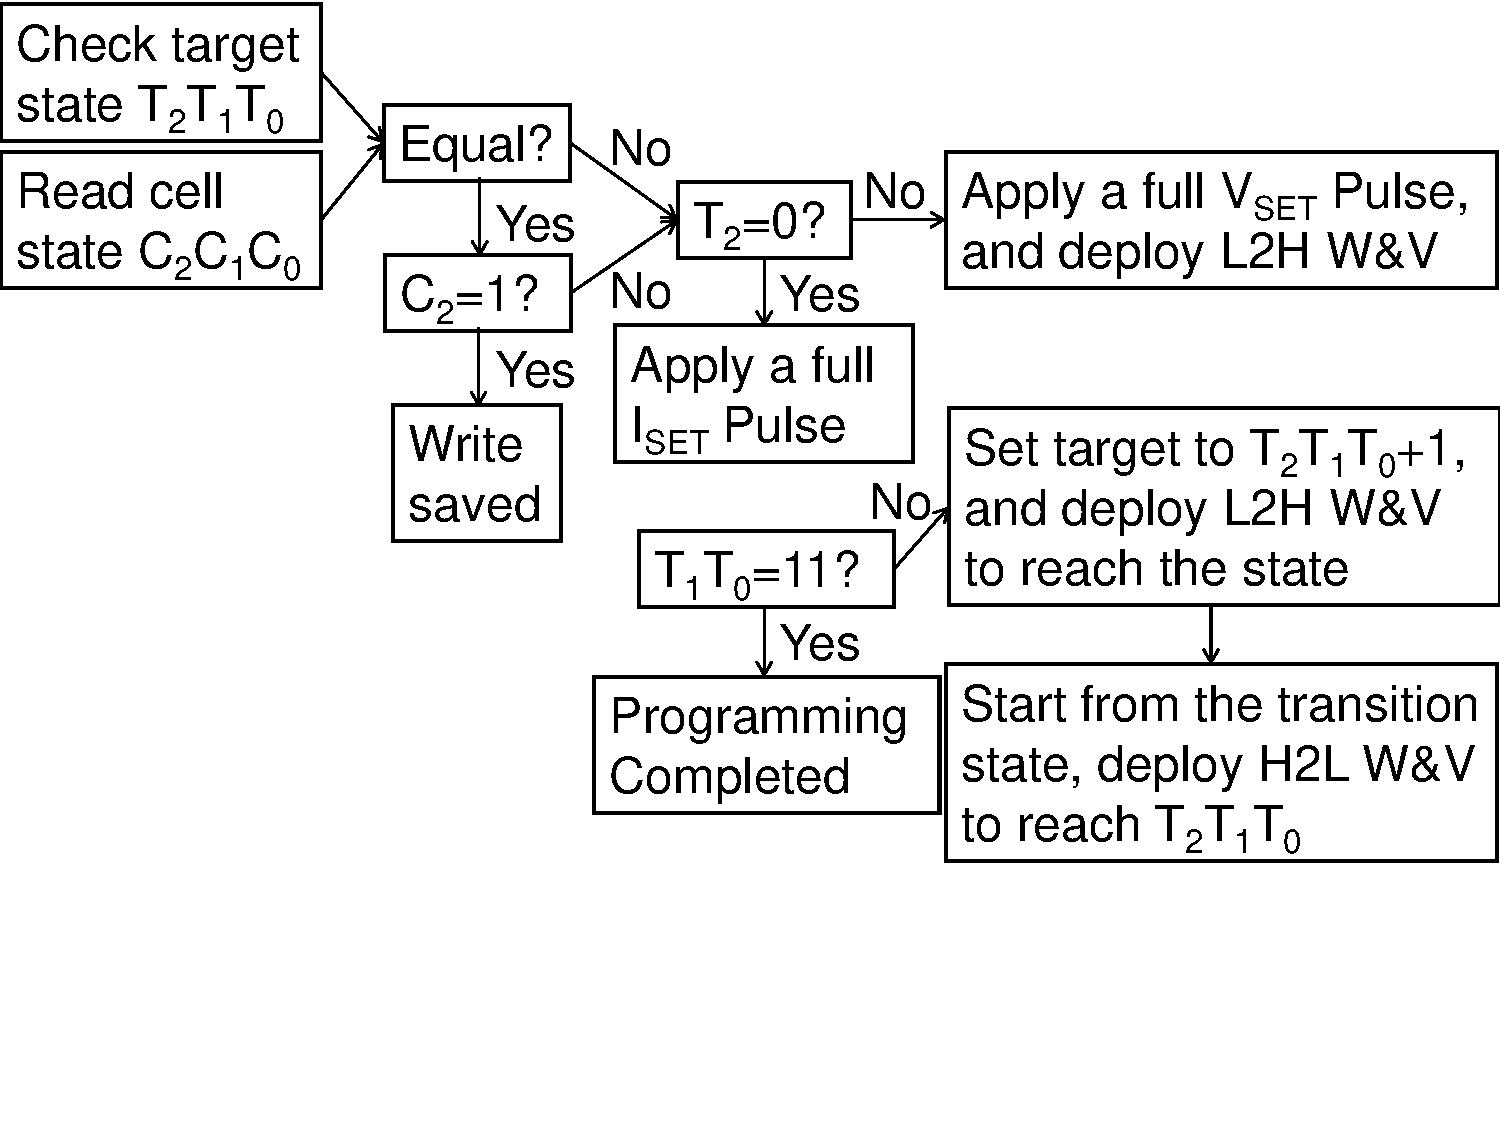
\includegraphics[width=0.48\textwidth]{fig/reliableprog}
\vspace{-10pt}
\caption{Flowchart of reliable programming methodology}
\label{fig:reliableprog}
\vspace{-15pt}
\end{figure}

The goal of the reliable MLC programming methodology is to meet the retention requirement (i.e. $>$years) of the programmed states by associating LRS with constructed strong CFs and HRS with ruptured weak CFs. The flowchart of the proposed programming methodology is illustrated in Figure~\ref{fig:reliableprog}. In reliable programming methodology, write operation is only saved if the target state is relative low resistance and equal to the original cell state when existing strong CFs are guaranteed in LRS. If the target state is relative low resistance but not equal to the original cell state, then a complete SET operation is performed 

